\chapter{Keyword Spotting and Voice Activity Detection}

\section{Introduction}

We propose a single neural network architecture to accomplish three tasks:
large-vocabulary continuous speech recognition (LVCSR), on-line keyword
spotting (KWS), and voice activity detection (VAD). The model is based on work
in end-to-end speech recognition which uses the Connectionist Temporal
Classification loss function coupled with deep Recurrent Neural Networks
\cite{graves2014, hannun2014deepspeech}. In this work we develop the model and
inference procedure for the KWS and VAD tasks. A thorough treatment of the
benefits of this model for LVCSR is given in \cite{amodei2016deep}.

One of the main benefits in using the same architecture for all three tasks is
simplicity. We need to maintain only a single architecture for training and
deployment of the ASR, KWS and VAD model. We literally use the same model
parameters for the KWS and VAD tasks. Given that these models run on-device,
this can be a considerable space saving. However, as we show our model also
achieves high accuracy on the VAD and KWS tasks. 

Like in LVCSR, adopting a more end-to-end approach to the tasks of KWS and VAD
also reduces the number of components needed to train the model. We are able to
train LVCSR, KWS and VAD models without needing to bootstrap an alignment of
output class labels to input frames. Furthermore we do not require the use of a
pronunciation dictionary or models to build context-dependent output classes.

Many competing methods exist for KWS. Sometimes a lightweight model is needed
which can run in real-time on a smart phone with a small memory footprint
without draining the battery life. In other tasks a more heavyweight model can
be used server side as an `audiogrep' tool. In some cases the application needs
to detect a single word or combination of words (e.g. ``Ok Google") with high
accuracy. In other instances the application needs to search a list of words
from a given vocabulary and allow the end-user to choose the keyword. In VAD, a
super lightweight model is typically needed which can run as a background
process on a sleeping smart phone for many hours without draining the battery.
However, occasionally a larger model can be used on a plugged in device (e.g.
the Amazon Echo) or server-side for end-pointing an utterance.

We specifically consider the task of on-line KWS on embedded devices - commonly
referred to as a ``wake word". For the VAD we are mostly focused on determining
when a user has finished speaking, a task often referred to as end-pointing.
The constraints for this model are that it must fit on the smart phone and be
able to run efficiently while the application is active. For the use-cases we
consider this tends to be around an hour. However, the model we describe is
general in the sense that the hyper-parameters can tuned such that one can
trade-off accuracy and computational efficiency for any of the above tasks.

A model which fits our power and latency constraints (about 600K parameters) to
be deployed on an iPhone 6 achieves a true positive rate of 94.9\% for a 0.6\%
false positive rate in detecting the keyword ``Olivia". For the VAD task the
same model achieves a 99.9\% true positive rate at a 5.0\% false positive rate
when labelling a full utterance as containing speech or not.

\section{Related Work}
\label{sec:kws:related}

Recently, research in Automatic Speech Recognition (ASR) has trended towards
more ``end-to-end" models~\cite{hannun2014deepspeech, chan2016, chorowski2015}.
These models do not require an alignment of class labels to audio input frames
to train. Often they output directly to characters~\cite{hannun2014deepspeech}
and even whole words \cite{chan2016} and read from the input waveform
directly~\cite{zhu2016}.

Here we explore the question of how to leverage this work for the tasks of
Keyword Spotting and Voice Activity Detection. Intuitively, model architectures
which work well for large vocabulary speech recognizers should also be useful
for these simpler speech tasks. 

Keyword spotting like LVCSR is generally done with an HMM to model the
probability of the observation sequence given the hidden state sequence of the
label~\cite{rohlicek1990, rose1990}. One can threshold the ratio of this
probability to that of a filler HMM to tune false negatives for a given false
positive rate. Like in LVCSR, one can substitute a DNN to compute the emission
probabilities of the HMM instead of a GMM.

Recently, to solve the KWS task a variety of models have been proposed, most of
which diverge from the usual ASR system. One method uses a bi-directional LSTM
which outputs to whole keyword units~\cite{fernandez2007}. The model is trained
with CTC and does not need an alignment of the keyword to the audio input.
However, this model has to be trained from scratch every time a new keyword is
added or the wake word is changed. Furthermore, outputting to whole keyword
units is not the most efficient use of the speech corpus. For example if we
want to learn the keyword ``okay sam" we would like to be able to leverage all
utterances that have ``okay" or ``sam" present regardless if the two words
occur consecutively. Another method uses a DNN to predict the words of a
keyword. The data is aligned using a large vocabulary speech
recognizer~\cite{chen2014}. A custom scoring function operates on windows of
outputs produced from the DNN in order to predict the presence of a key-word.  

In these methods either an alignment is needed or the model outputs directly to
keyword units. In contrast our model does not require the alignment of the
transcript to the audio since we use the CTC cost function. Also since the
model outputs to characters directly, we are able to better leverage the data
and quickly adapt the model to new keywords.

Models for voice activity detection (VAD) have a wide range of complexity. Some
simple and efficient techniques include a threshold on the energy of the audio
signal, a threshold on the number of zero-crossings~\cite{junqua1991} or
classifiers built from combinations of these features. Speech typically has
higher energy than non-speech noise and fewer zero-crossings. These methods are
typically not robust to non-stationary environments. More complex parameter
estimation methods work better. A model resembling HMM-GMM ASR can be used. In
this model a Gaussian represents the non-speech distribution and another
represents the speech distribution~\cite{sohn1999}. An HMM is typically applied
on top of these observation probabilities to smooth the estimates over time. A
unique RNN architecture has also been shown to work well for
VAD~\cite{hughes2013}. 

In the parameter estimation methods used for VAD, a corpus of audio frames
labeled as speech or non-speech is needed. This corpus is typically produced
with a forced-alignment from a large vocabulary ASR system. 

\section{Model}
\label{sec:kws:model}

For a general keyword spotter we need a model which can give us $p(k | x)$
where $x$ is a window of speech and $k$ is any keyword. For VAD we use the same
distribution and simply set $k$ to the empty string.

We use the Connectionist Temporal Classification~\cite{graves2006} (CTC)
objective function to train an RNN on a corpus of utterance and transcription
pairs. The CTC objective gives us the probability of any label string for a
given utterance. We do not need an alignment here because CTC efficiently
computes the score over all possible alignments. The objective function for an
utterance $x$ and corresponding transcription $\ell$ is given by
\begin{equation}
p_{\mathrm{CTC}}(\ell | x) = \sum_{s \in \mathrm{align}(\ell, T)} \prod_t^T p(s_t | x).
\end{equation}
The $\mathrm{align}(\cdot)$ function computes the set of possible alignments of
the transcription $\ell$ over the $T$ time-steps of the utterance under the CTC
operator. The CTC operator allows for repetitions of any character and
insertions of the blank character, $\epsilon$, which signifies no output at a
given time-step.

For the on-line KWS task we must determine with low latency if the keyword has
been said. Thus, in order to use this model for KWS we score a moving window of
the audio stream $x$ so that we can find the keyword soon after it occurs. The
score is computed as $p_{\mathrm{CTC}}(k | x_{t:t+w})$ where $k$ is any keyword
and $x_{t:t+w}$ is a window of speech $w$ frames long. For the VAD task we
first compute the probability of no speech by setting $k$ to the empty string.
From this we can find the probability of speech by taking one minus the
probability of no speech.

\subsection{Network Architecture}
\label{sec:kws:architecture}

The network accepts as input a spectrogram computed from the raw waveform
sampled at 8kHz. The first layer is a 2-dimensional convolution with a stride
of three~\cite{amodei2016deep}. For the next three layers of the network we use
gated recurrent RNN layers~\cite{cho2014} as they typically work as well as an
LSTM but are more efficient~\cite{chung2014}. The last layer is a single affine
transformation followed by a softmax. The network outputs directly to
characters in the alphabet including the blank and space characters.

\subsection{Inference}

In practice, as is typical of most KWS models, one has to choose a window size
of speech over which to evaluate the possibility of the keyword being present.
The accuracy of the algorithm can be sensitive to this parameter. If the window
size is too small, then the entire keyword may not have been seen. On the other
hand, if the window size is too large, other speech may be present and since
our model evaluates the presence of only the keyword this can be problematic.
We do not want to limit what the user can say directly before or after the
keyword. In fact, allowing the user to talk-through the wake word without
needing to pause between it and the actual utterance gives a more natural
experience. Setting the window size parameter can be tricky given that the
keyword can be realized in many different lengths depending on the rate of
speech of the user.

To alleviate the sensitivity of the algorithm to the window size parameter we
propose a modification to the CTC scoring algorithm presented above. For a
given keyword $k$ instead of scoring $k$ under the model we instead score the
regular expression [\^{}$k_0$]*$k$[\^{}$k_{n-1}$]*, where $k_0$ and $k_{n-1}$
are the first and last characters of $k$. An implementation for computing this
modified CTC score is shown in Algorithm \ref{alg:kws:scorekeyword}.

\begin{algorithm}
\caption{Computing the score of a keyword, $k$, given the output probabilities
         of the RNN. The algorithm accepts $l$ and $P$ as parameters. The variable
         $l$ is the keyword with $\epsilon$ inserted at the beginning, end and
         between every pair of characters of $k$. The matrix $P$ contains the
         distributions over output characters in its columns for each time-step.}
\label{alg:scorekeyword}
\begin{algorithmic}
\Function{ScoreKeyword}{$l$, $P$}
\State $S$ $\gets$ size($l$)
\State $T$ $\gets$ numberOfColumns($P$)
\State $\alpha \gets$ zeros(S, T)
\State $\alpha_{1, 1} \gets 1 - P_{l_2, 1}$
\State $\alpha_{2, 1} \gets P_{l_{2}, 1}$
    \For{$t=2:T$}
        \For{$s=1:S$}
            \If{$s = 1$}
                \State $p \gets 1 - P_{l_2, t}$
            \ElsIf{$s = S$}
                \State $p \gets 1 - P_{l_{S - 1}, t}$
            \Else
                \State $p \gets P_{l_{s}, t}$
            \EndIf
            
            \If{$s > 2$ and $l_s \ne l_{s-2}$ and $l_s \ne \epsilon$}
                \State $\alpha_{s, t} \gets p * (\alpha_{s, t-1} + \alpha_{s-1, t-1} + \alpha_{s-2, t-1})$
            \ElsIf {$s > 1$}
                \State $\alpha_{s, t} \gets p * (\alpha_{s, t-1} + \alpha_{s-1, t-1})$
            \Else
                \State $\alpha_{s, t} \gets p * \alpha_{s, t-1}$
            \EndIf
        \EndFor
    \EndFor
    \State \Return $\alpha_{S, T} + \alpha_{S-1, T}$
\EndFunction
\end{algorithmic}
\end{algorithm}

Algorithm \ref{alg:kws:scorekeyword} allows us to choose a window size long
enough such that all occurrences of the keyword are shorter than it and not
worry if other speech is present before or after the keyword.

Computing the VAD score is efficient as it reduces to summing the log
probabilities of the blank character over the window of speech frames
\begin{equation}
\log p(\mathrm{speech}| x_{t:t+w}) = 1 - \sum_{i=t}^{t + w} \log p_i(\epsilon | x_{t:t+w}).
\end{equation}

\section{Experiments}
\label{sec:kws:experiments}

In this section we show several experiments evaluating the model for both the
KWS and VAD task. We explore the performance of the model varying the number of
layers, layer sizes and data used to train the system.

The model parameters are optimizes with stochastic gradient descent. All models
are trained for 50 epochs where an epoch is a full pass through the data. The
learning rate and momentum parameters are chosen to optimize speed of
convergence. We anneal the learning rate by a factor of 0.9 every 5000
iterations. All experiments use a minibatch of 256 examples during training. We
sort examples so that the minibatch consists of utterances of similar length
for computational efficiency. 

The architecture of the network is as described in
Section~\ref{sec:kws:architecture}. The filters for the convolution layer are
11 by 32 over the time and frequency dimensions respectively. We use 32 filters
in all models.

The data used to train the model consists of two data-sets. The first data-set
is a corpus 526K transcribed utterances collected on Android phones via an
assistant like application. The second corpus consists of 1544 spoken examples
of the name ``Olivia'', the keyword we want the model to recognize. The model
is trained on both data-sets simultaneously. We do not need to pre-train on the
large corpus prior to fine-tuning. We also use a collection of about a hundred
hours of noise and music downloaded from the web to generate synthetic noisy
examples of the keyword and empty noise clips. When training with the noisy
data we replicate each keyword 10 times, each time with a random noise clip. We
also use a corpus of 57K randomly sampled noise clips with a blank label as
filler.

The KWS model is evaluated on a test set of 550 positive examples (e.g.
containing the keyword ``Olivia``) and 5000 negative examples held-out from the
large speech corpus described above. During inference we evaluate the utterance
with Algorithm~\ref{alg:kws:scorekeyword} every 100 milliseconds over a window
of 800 milliseconds in order to detect the presence of the keyword. We classify
an example as positive if the score found from the output of
Algorithm~\ref{alg:kws:scorekeyword} over the utterance is ever above a preset
threshold.  In the results shown below we plot ROC curves with the False
Positive rate on the horizontal axis and the True Positive rate on the vertical
axis.

We evaluate the same models on the VAD task. The positive examples are the same
5000 examples of speech used as the negative examples for the KWS task. We
collected about 10 hours of non-speech audio from a variety of noise
backgrounds. We sample 5000 random clips from the 10 hours of noise to
construct the negative samples.

Figures \ref{fig:kws:layers} and \ref{fig:kws:sizes} show that the model
consistently improves at detecting the keyword as we increase the number of
layers and the size of the model. In the KWS task we are constrained by
computational resources. However, these results suggests that a promising
direction for improving KWS performance is to find ways to deploy larger models
more efficiently. 

In the VAD task increasing the model depth does consistently improve
performance. Similarly, increasing the layer size only helps up to a point.
After the layers are larger than 128 units, the performance saturates. For most
of the VAD models achieve near 99.9\% true positive rate or higher at a fixed
false positive rate of 5.0\%.

\begin{figure}
\centering
\begin{subfigure}{0.47\textwidth}
    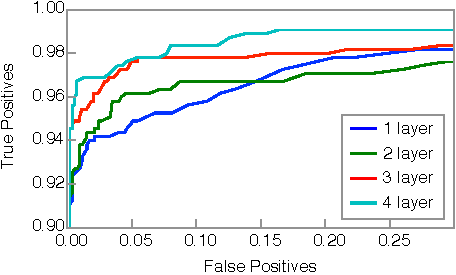
\includegraphics[width=\textwidth]{kws/figures/layers.pdf}
    \caption{KWS}
\end{subfigure}
\hfill
\begin{subfigure}{0.47\textwidth}
    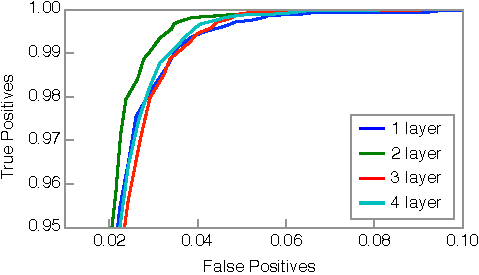
\includegraphics[width=\textwidth]{kws/figures/layers_vad.pdf}
    \caption{VAD}
\end{subfigure}
\caption{The performance of the model on both the KWS and VAD
         tasks varying the number of hidden layers from 1 to 4. The layer size for
         all models is fixed at 256 hidden units.}
\label{fig:kws:layers} 
\end{figure}

\begin{figure}
\centering
\begin{subfigure}{0.47\textwidth}
    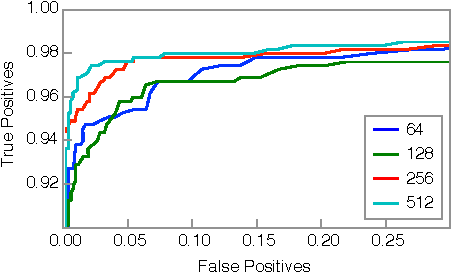
\includegraphics[width=\textwidth]{kws/figures/sizes.pdf}
    \caption{KWS}
\end{subfigure}
\hfill
\begin{subfigure}{0.47\textwidth}
    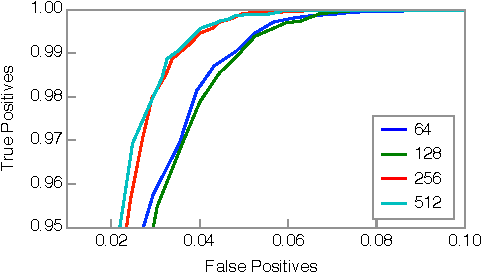
\includegraphics[width=\textwidth]{kws/figures/sizes_vad.pdf}
    \caption{VAD}
\end{subfigure}
\caption{The performance of the model on both the KWS and VAD tasks varying the
         layer size from 64 to 512. The number of hidden layers for all models is
         fixed at 3.}
\label{fig:kws:sizes} 
\end{figure}

In Figure~\ref{fig:kws:data} we see that adding noise to the keywords during
training results in substantial improvements. At a false positive rate of 1\%
the model with noise has a true positive rate of 95.8\% compared to 87.2\% for
the model without noise. Further using the random noise data on its own does
not help much; in fact the results are slightly worse. On the VAD task we also
notice an improvement in the ROC curve as we add noise. However, the
improvement in VAD is not nearly as significant as in KWS.

\begin{figure}
\centering
\begin{subfigure}{0.47\textwidth}
    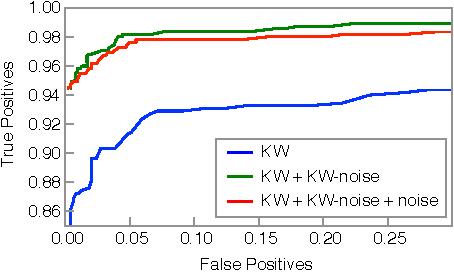
\includegraphics[width=\textwidth]{kws/figures/data.pdf}
    \caption{KWS}
\end{subfigure}
\hfill
\begin{subfigure}{0.47\textwidth}
    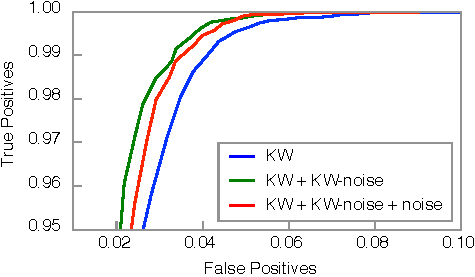
\includegraphics[width=\textwidth]{kws/figures/data_vad.pdf}
    \caption{VAD}
\end{subfigure}
\caption{The performance of the model on both the KWS and VAD tasks as we add
         training data. The `KW' model does not have any noise synthesis but does
         contain the 550K filler examples. The `KW + KW noise' model includes
         the keyword data replicated 10 times with random noise. The `KW + KW noise
         + noise' includes 57K random noise clips as filler.}
\label{fig:kws:data} 
\end{figure}

\section{Conclusion}
\label{sec:kws:conclusion}

We have described a single neural network architecture which can be used for
accurate large vocabulary speech recognition, key word spotting and voice
activity detection. The model is simple to train and does not require an
alignment or frame-wise labels. One only needs a large speech corpus with the
corresponding transcriptions. We also give the details of an inference
algorithm for KWS modified from the basic CTC scoring algorithm.

As our experiments have demonstrated, further improvement on the KWS task can
come from better fitting the training data. Given the power and memory
constraints of a deployed KWS and VAD model, finding ways to improve the
efficiency of more expressive models will be a useful direction.
